

\tikzset{every picture/.style={line width=0.75pt}} %set default line width to 0.75pt        

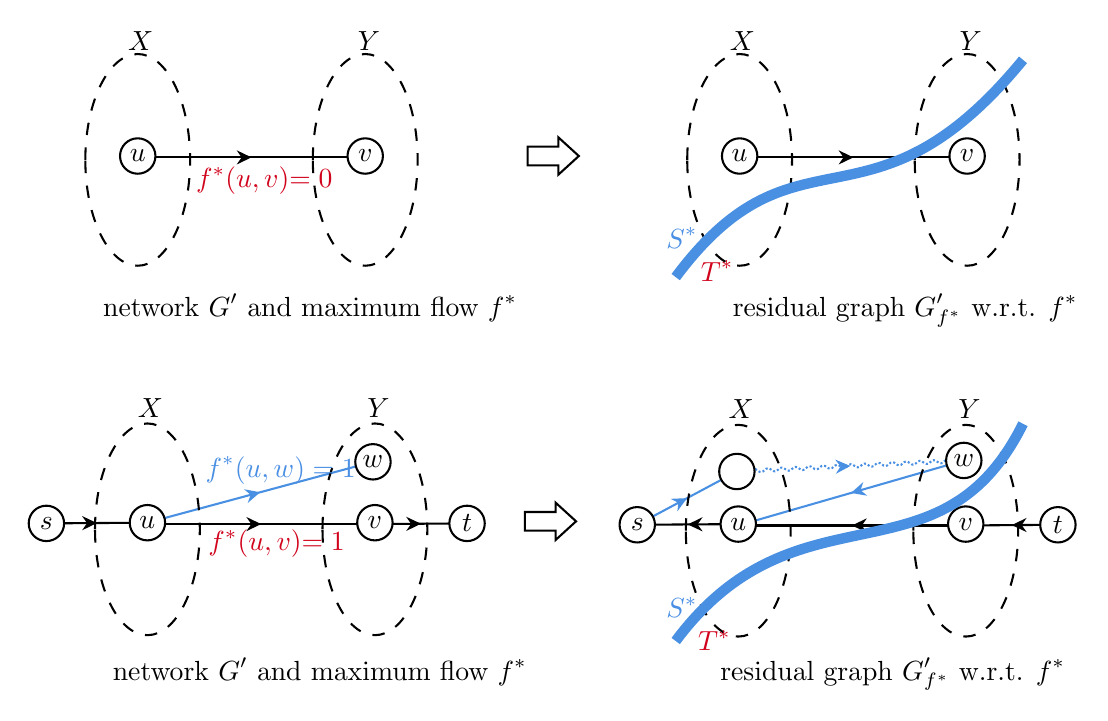
\begin{tikzpicture}[x=0.5pt,y=0.5pt,yscale=-1,xscale=1]
%uncomment if require: \path (0,489); %set diagram left start at 0, and has height of 489

%Straight Lines [id:da6191213399358775] 
\draw [color={rgb, 255:red, 74; green, 144; blue, 226 }  ,draw opacity=1 ]   (256.22,322.5) -- (93.22,366.5) ;
\draw [shift={(174.72,344.5)}, rotate = 164.89] [fill={rgb, 255:red, 74; green, 144; blue, 226 }  ,fill opacity=1 ][line width=0.08]  [draw opacity=0] (10.72,-5.15) -- (0,0) -- (10.72,5.15) -- (7.12,0) -- cycle    ;
%Straight Lines [id:da8327265709083349] 
\draw [color={rgb, 255:red, 74; green, 144; blue, 226 }  ,draw opacity=1 ]   (447.22,368) -- (519.22,329.5) ;
\draw [shift={(483.22,348.75)}, rotate = 511.87] [fill={rgb, 255:red, 74; green, 144; blue, 226 }  ,fill opacity=1 ][line width=0.08]  [draw opacity=0] (10.72,-5.15) -- (0,0) -- (10.72,5.15) -- (7.12,0) -- cycle    ;
%Straight Lines [id:da8516915581936988] 
\draw [color={rgb, 255:red, 74; green, 144; blue, 226 }  ,draw opacity=1 ] [dash pattern={on 0.75pt off 0.75pt}]  (519.22,329.5) .. controls (520.8,327.76) and (522.46,327.68) .. (524.21,329.26) .. controls (525.96,330.85) and (527.62,330.77) .. (529.21,329.02) .. controls (530.79,327.27) and (532.45,327.19) .. (534.2,328.77) .. controls (535.95,330.36) and (537.61,330.28) .. (539.19,328.53) .. controls (540.78,326.78) and (542.44,326.7) .. (544.19,328.29) .. controls (545.94,329.87) and (547.6,329.79) .. (549.18,328.04) .. controls (550.77,326.29) and (552.43,326.21) .. (554.18,327.8) .. controls (555.93,329.39) and (557.59,329.31) .. (559.17,327.56) .. controls (560.76,325.81) and (562.42,325.73) .. (564.17,327.31) .. controls (565.92,328.9) and (567.58,328.82) .. (569.16,327.07) .. controls (570.74,325.32) and (572.4,325.24) .. (574.15,326.83) .. controls (575.9,328.41) and (577.56,328.33) .. (579.15,326.58) .. controls (580.73,324.83) and (582.39,324.75) .. (584.14,326.34) .. controls (585.89,327.92) and (587.55,327.84) .. (589.14,326.09) .. controls (590.72,324.34) and (592.38,324.26) .. (594.13,325.85) .. controls (595.88,327.44) and (597.54,327.36) .. (599.12,325.61) .. controls (600.71,323.86) and (602.37,323.78) .. (604.12,325.36) .. controls (605.87,326.95) and (607.53,326.87) .. (609.11,325.12) .. controls (610.7,323.37) and (612.36,323.29) .. (614.11,324.88) .. controls (615.86,326.46) and (617.52,326.38) .. (619.1,324.63) .. controls (620.68,322.88) and (622.34,322.8) .. (624.09,324.39) .. controls (625.84,325.98) and (627.5,325.9) .. (629.09,324.15) .. controls (630.67,322.4) and (632.33,322.32) .. (634.08,323.9) .. controls (635.83,325.49) and (637.49,325.41) .. (639.08,323.66) .. controls (640.66,321.91) and (642.32,321.83) .. (644.07,323.41) .. controls (645.82,325) and (647.48,324.92) .. (649.06,323.17) .. controls (650.65,321.42) and (652.31,321.34) .. (654.06,322.93) .. controls (655.81,324.51) and (657.47,324.43) .. (659.05,322.68) .. controls (660.64,320.93) and (662.3,320.85) .. (664.05,322.44) .. controls (665.8,324.03) and (667.46,323.95) .. (669.04,322.2) .. controls (670.62,320.45) and (672.28,320.37) .. (674.03,321.95) .. controls (675.78,323.54) and (677.44,323.46) .. (679.03,321.71) -- (683.22,321.5) -- (683.22,321.5) ;
\draw [shift={(601.22,325.5)}, rotate = 537.21] [fill={rgb, 255:red, 74; green, 144; blue, 226 }  ,fill opacity=1 ][line width=0.08]  [draw opacity=0] (10.72,-5.15) -- (0,0) -- (10.72,5.15) -- (7.12,0) -- cycle    ;
%Straight Lines [id:da8322109543199766] 
\draw [color={rgb, 255:red, 74; green, 144; blue, 226 }  ,draw opacity=1 ]   (683.22,321.5) -- (520.22,368.5) ;
\draw [shift={(601.72,345)}, rotate = 343.91999999999996] [fill={rgb, 255:red, 74; green, 144; blue, 226 }  ,fill opacity=1 ][line width=0.08]  [draw opacity=0] (10.72,-5.15) -- (0,0) -- (10.72,5.15) -- (7.12,0) -- cycle    ;
%Straight Lines [id:da577325970602598] 
\draw    (250.62,102.5) -- (86.22,102.5) ;
\draw [shift={(168.42,102.5)}, rotate = 180] [fill={rgb, 255:red, 0; green, 0; blue, 0 }  ][line width=0.08]  [draw opacity=0] (10.72,-5.15) -- (0,0) -- (10.72,5.15) -- (7.12,0) -- cycle    ;
%Shape: Ellipse [id:dp513666224672568] 
\draw  [fill={rgb, 255:red, 255; green, 255; blue, 255 }  ,fill opacity=1 ] (73.43,101.5) .. controls (73.43,94.44) and (79.15,88.71) .. (86.22,88.71) .. controls (93.28,88.71) and (99.01,94.44) .. (99.01,101.5) .. controls (99.01,108.57) and (93.28,114.29) .. (86.22,114.29) .. controls (79.15,114.29) and (73.43,108.57) .. (73.43,101.5) -- cycle ;
%Shape: Ellipse [id:dp9236001904458527] 
\draw  [fill={rgb, 255:red, 255; green, 255; blue, 255 }  ,fill opacity=1 ] (237.83,101.5) .. controls (237.83,94.44) and (243.56,88.71) .. (250.62,88.71) .. controls (257.69,88.71) and (263.41,94.44) .. (263.41,101.5) .. controls (263.41,108.57) and (257.69,114.29) .. (250.62,114.29) .. controls (243.56,114.29) and (237.83,108.57) .. (237.83,101.5) -- cycle ;
%Right Arrow [id:dp2218646176992478] 
\draw   (368,94.75) -- (390.2,94.75) -- (390.2,88) -- (405,101.5) -- (390.2,115) -- (390.2,108.25) -- (368,108.25) -- cycle ;
%Shape: Ellipse [id:dp7576706437482376] 
\draw  [dash pattern={on 4.5pt off 4.5pt}] (48.34,104.29) .. controls (48.34,62.04) and (65.3,27.79) .. (86.22,27.79) .. controls (107.14,27.79) and (124.09,62.04) .. (124.09,104.29) .. controls (124.09,146.54) and (107.14,180.79) .. (86.22,180.79) .. controls (65.3,180.79) and (48.34,146.54) .. (48.34,104.29) -- cycle ;
%Shape: Ellipse [id:dp019919118199761776] 
\draw  [dash pattern={on 4.5pt off 4.5pt}] (212.75,104.29) .. controls (212.75,62.04) and (229.7,27.79) .. (250.62,27.79) .. controls (271.54,27.79) and (288.5,62.04) .. (288.5,104.29) .. controls (288.5,146.54) and (271.54,180.79) .. (250.62,180.79) .. controls (229.7,180.79) and (212.75,146.54) .. (212.75,104.29) -- cycle ;
%Straight Lines [id:da8311742548484229] 
\draw    (685.62,102.5) -- (521.22,102.5) ;
\draw [shift={(603.42,102.5)}, rotate = 180] [fill={rgb, 255:red, 0; green, 0; blue, 0 }  ][line width=0.08]  [draw opacity=0] (10.72,-5.15) -- (0,0) -- (10.72,5.15) -- (7.12,0) -- cycle    ;
%Shape: Ellipse [id:dp9405415347638398] 
\draw  [fill={rgb, 255:red, 255; green, 255; blue, 255 }  ,fill opacity=1 ] (508.43,101.5) .. controls (508.43,94.44) and (514.15,88.71) .. (521.22,88.71) .. controls (528.28,88.71) and (534.01,94.44) .. (534.01,101.5) .. controls (534.01,108.57) and (528.28,114.29) .. (521.22,114.29) .. controls (514.15,114.29) and (508.43,108.57) .. (508.43,101.5) -- cycle ;
%Shape: Ellipse [id:dp11646647893691375] 
\draw  [fill={rgb, 255:red, 255; green, 255; blue, 255 }  ,fill opacity=1 ] (672.83,101.5) .. controls (672.83,94.44) and (678.56,88.71) .. (685.62,88.71) .. controls (692.69,88.71) and (698.41,94.44) .. (698.41,101.5) .. controls (698.41,108.57) and (692.69,114.29) .. (685.62,114.29) .. controls (678.56,114.29) and (672.83,108.57) .. (672.83,101.5) -- cycle ;
%Shape: Ellipse [id:dp9449855279419199] 
\draw  [dash pattern={on 4.5pt off 4.5pt}] (483.34,104.29) .. controls (483.34,62.04) and (500.3,27.79) .. (521.22,27.79) .. controls (542.14,27.79) and (559.09,62.04) .. (559.09,104.29) .. controls (559.09,146.54) and (542.14,180.79) .. (521.22,180.79) .. controls (500.3,180.79) and (483.34,146.54) .. (483.34,104.29) -- cycle ;
%Shape: Ellipse [id:dp97494012923029] 
\draw  [dash pattern={on 4.5pt off 4.5pt}] (647.75,104.29) .. controls (647.75,62.04) and (664.7,27.79) .. (685.62,27.79) .. controls (706.54,27.79) and (723.5,62.04) .. (723.5,104.29) .. controls (723.5,146.54) and (706.54,180.79) .. (685.62,180.79) .. controls (664.7,180.79) and (647.75,146.54) .. (647.75,104.29) -- cycle ;
%Straight Lines [id:da25721893854693145] 
\draw    (93.22,366.5) -- (20.22,367) ;
\draw [shift={(56.72,366.75)}, rotate = 179.61] [fill={rgb, 255:red, 0; green, 0; blue, 0 }  ][line width=0.08]  [draw opacity=0] (10.72,-5.15) -- (0,0) -- (10.72,5.15) -- (7.12,0) -- cycle    ;
%Straight Lines [id:da4797079273399141] 
\draw    (324.22,367) -- (257.62,367.5) ;
\draw [shift={(290.92,367.25)}, rotate = 179.57] [fill={rgb, 255:red, 0; green, 0; blue, 0 }  ][line width=0.08]  [draw opacity=0] (10.72,-5.15) -- (0,0) -- (10.72,5.15) -- (7.12,0) -- cycle    ;
%Straight Lines [id:da0639605968996434] 
\draw    (257.62,367.5) -- (93.22,367.5) ;
\draw [shift={(175.42,367.5)}, rotate = 180] [fill={rgb, 255:red, 0; green, 0; blue, 0 }  ][line width=0.08]  [draw opacity=0] (10.72,-5.15) -- (0,0) -- (10.72,5.15) -- (7.12,0) -- cycle    ;
%Shape: Ellipse [id:dp7215149302709682] 
\draw  [fill={rgb, 255:red, 255; green, 255; blue, 255 }  ,fill opacity=1 ] (80.43,366.5) .. controls (80.43,359.44) and (86.15,353.71) .. (93.22,353.71) .. controls (100.28,353.71) and (106.01,359.44) .. (106.01,366.5) .. controls (106.01,373.57) and (100.28,379.29) .. (93.22,379.29) .. controls (86.15,379.29) and (80.43,373.57) .. (80.43,366.5) -- cycle ;
%Shape: Ellipse [id:dp10876362413389085] 
\draw  [fill={rgb, 255:red, 255; green, 255; blue, 255 }  ,fill opacity=1 ] (244.83,366.5) .. controls (244.83,359.44) and (250.56,353.71) .. (257.62,353.71) .. controls (264.69,353.71) and (270.41,359.44) .. (270.41,366.5) .. controls (270.41,373.57) and (264.69,379.29) .. (257.62,379.29) .. controls (250.56,379.29) and (244.83,373.57) .. (244.83,366.5) -- cycle ;
%Shape: Ellipse [id:dp34296507659419695] 
\draw  [dash pattern={on 4.5pt off 4.5pt}] (55.34,371.29) .. controls (55.34,329.04) and (72.3,294.79) .. (93.22,294.79) .. controls (114.14,294.79) and (131.09,329.04) .. (131.09,371.29) .. controls (131.09,413.54) and (114.14,447.79) .. (93.22,447.79) .. controls (72.3,447.79) and (55.34,413.54) .. (55.34,371.29) -- cycle ;
%Shape: Ellipse [id:dp8298689489920419] 
\draw  [dash pattern={on 4.5pt off 4.5pt}] (219.75,371.29) .. controls (219.75,329.04) and (236.7,294.79) .. (257.62,294.79) .. controls (278.54,294.79) and (295.5,329.04) .. (295.5,371.29) .. controls (295.5,413.54) and (278.54,447.79) .. (257.62,447.79) .. controls (236.7,447.79) and (219.75,413.54) .. (219.75,371.29) -- cycle ;
%Shape: Ellipse [id:dp9137920481521634] 
\draw  [fill={rgb, 255:red, 255; green, 255; blue, 255 }  ,fill opacity=1 ] (7.43,367) .. controls (7.43,359.94) and (13.15,354.21) .. (20.22,354.21) .. controls (27.28,354.21) and (33.01,359.94) .. (33.01,367) .. controls (33.01,374.07) and (27.28,379.79) .. (20.22,379.79) .. controls (13.15,379.79) and (7.43,374.07) .. (7.43,367) -- cycle ;
%Shape: Ellipse [id:dp215960632133124] 
\draw  [fill={rgb, 255:red, 255; green, 255; blue, 255 }  ,fill opacity=1 ] (311.43,367) .. controls (311.43,359.94) and (317.15,354.21) .. (324.22,354.21) .. controls (331.28,354.21) and (337.01,359.94) .. (337.01,367) .. controls (337.01,374.07) and (331.28,379.79) .. (324.22,379.79) .. controls (317.15,379.79) and (311.43,374.07) .. (311.43,367) -- cycle ;
%Curve Lines [id:da39738584929269916] 
\draw [color={rgb, 255:red, 74; green, 144; blue, 226 }  ,draw opacity=1 ][line width=3.75]    (475,189) .. controls (563,71) and (615,167) .. (726,32) ;
%Straight Lines [id:da7379384720847889] 
\draw    (520.22,367.5) -- (447.22,368) ;
\draw [shift={(483.72,367.75)}, rotate = 359.61] [fill={rgb, 255:red, 0; green, 0; blue, 0 }  ][line width=0.08]  [draw opacity=0] (10.72,-5.15) -- (0,0) -- (10.72,5.15) -- (7.12,0) -- cycle    ;
%Straight Lines [id:da3670804661459104] 
\draw    (751.22,368) -- (684.62,368.5) ;
\draw [shift={(717.92,368.25)}, rotate = 359.57] [fill={rgb, 255:red, 0; green, 0; blue, 0 }  ][line width=0.08]  [draw opacity=0] (10.72,-5.15) -- (0,0) -- (10.72,5.15) -- (7.12,0) -- cycle    ;
%Straight Lines [id:da21692742405585586] 
\draw    (684.62,368.5) -- (520.22,368.5) ;
\draw [shift={(602.42,368.5)}, rotate = 360] [fill={rgb, 255:red, 0; green, 0; blue, 0 }  ][line width=0.08]  [draw opacity=0] (10.72,-5.15) -- (0,0) -- (10.72,5.15) -- (7.12,0) -- cycle    ;
%Shape: Ellipse [id:dp4921121681649563] 
\draw  [fill={rgb, 255:red, 255; green, 255; blue, 255 }  ,fill opacity=1 ] (507.43,367.5) .. controls (507.43,360.44) and (513.15,354.71) .. (520.22,354.71) .. controls (527.28,354.71) and (533.01,360.44) .. (533.01,367.5) .. controls (533.01,374.57) and (527.28,380.29) .. (520.22,380.29) .. controls (513.15,380.29) and (507.43,374.57) .. (507.43,367.5) -- cycle ;
%Shape: Ellipse [id:dp4020136360807661] 
\draw  [fill={rgb, 255:red, 255; green, 255; blue, 255 }  ,fill opacity=1 ] (671.83,367.5) .. controls (671.83,360.44) and (677.56,354.71) .. (684.62,354.71) .. controls (691.69,354.71) and (697.41,360.44) .. (697.41,367.5) .. controls (697.41,374.57) and (691.69,380.29) .. (684.62,380.29) .. controls (677.56,380.29) and (671.83,374.57) .. (671.83,367.5) -- cycle ;
%Shape: Ellipse [id:dp2784381633198203] 
\draw  [dash pattern={on 4.5pt off 4.5pt}] (482.34,372.29) .. controls (482.34,330.04) and (499.3,295.79) .. (520.22,295.79) .. controls (541.14,295.79) and (558.09,330.04) .. (558.09,372.29) .. controls (558.09,414.54) and (541.14,448.79) .. (520.22,448.79) .. controls (499.3,448.79) and (482.34,414.54) .. (482.34,372.29) -- cycle ;
%Shape: Ellipse [id:dp6984861741222058] 
\draw  [dash pattern={on 4.5pt off 4.5pt}] (646.75,372.29) .. controls (646.75,330.04) and (663.7,295.79) .. (684.62,295.79) .. controls (705.54,295.79) and (722.5,330.04) .. (722.5,372.29) .. controls (722.5,414.54) and (705.54,448.79) .. (684.62,448.79) .. controls (663.7,448.79) and (646.75,414.54) .. (646.75,372.29) -- cycle ;
%Shape: Ellipse [id:dp6691205194220659] 
\draw  [fill={rgb, 255:red, 255; green, 255; blue, 255 }  ,fill opacity=1 ] (434.43,368) .. controls (434.43,360.94) and (440.15,355.21) .. (447.22,355.21) .. controls (454.28,355.21) and (460.01,360.94) .. (460.01,368) .. controls (460.01,375.07) and (454.28,380.79) .. (447.22,380.79) .. controls (440.15,380.79) and (434.43,375.07) .. (434.43,368) -- cycle ;
%Shape: Ellipse [id:dp11182746749852701] 
\draw  [fill={rgb, 255:red, 255; green, 255; blue, 255 }  ,fill opacity=1 ] (738.43,368) .. controls (738.43,360.94) and (744.15,355.21) .. (751.22,355.21) .. controls (758.28,355.21) and (764.01,360.94) .. (764.01,368) .. controls (764.01,375.07) and (758.28,380.79) .. (751.22,380.79) .. controls (744.15,380.79) and (738.43,375.07) .. (738.43,368) -- cycle ;
%Curve Lines [id:da0028084380062078917] 
\draw [color={rgb, 255:red, 74; green, 144; blue, 226 }  ,draw opacity=1 ][line width=3.75]    (475,452) .. controls (563,334) and (666,416) .. (726,295) ;
%Shape: Ellipse [id:dp6641341242010522] 
\draw  [fill={rgb, 255:red, 255; green, 255; blue, 255 }  ,fill opacity=1 ] (506.43,329.5) .. controls (506.43,322.44) and (512.15,316.71) .. (519.22,316.71) .. controls (526.28,316.71) and (532.01,322.44) .. (532.01,329.5) .. controls (532.01,336.57) and (526.28,342.29) .. (519.22,342.29) .. controls (512.15,342.29) and (506.43,336.57) .. (506.43,329.5) -- cycle ;
%Shape: Ellipse [id:dp6412575212172368] 
\draw  [fill={rgb, 255:red, 255; green, 255; blue, 255 }  ,fill opacity=1 ] (670.43,321.5) .. controls (670.43,314.44) and (676.15,308.71) .. (683.22,308.71) .. controls (690.28,308.71) and (696.01,314.44) .. (696.01,321.5) .. controls (696.01,328.57) and (690.28,334.29) .. (683.22,334.29) .. controls (676.15,334.29) and (670.43,328.57) .. (670.43,321.5) -- cycle ;
%Shape: Ellipse [id:dp4382651677301832] 
\draw  [fill={rgb, 255:red, 255; green, 255; blue, 255 }  ,fill opacity=1 ] (243.43,322.5) .. controls (243.43,315.44) and (249.15,309.71) .. (256.22,309.71) .. controls (263.28,309.71) and (269.01,315.44) .. (269.01,322.5) .. controls (269.01,329.57) and (263.28,335.29) .. (256.22,335.29) .. controls (249.15,335.29) and (243.43,329.57) .. (243.43,322.5) -- cycle ;
%Right Arrow [id:dp9788576014249767] 
\draw   (366,358.75) -- (388.2,358.75) -- (388.2,352) -- (403,365.5) -- (388.2,379) -- (388.2,372.25) -- (366,372.25) -- cycle ;

% Text Node
\draw (250.62,101.5) node   [align=left] {$\displaystyle v$};
% Text Node
\draw (86.22,101.5) node   [align=left] {$\displaystyle u$};
% Text Node
\draw (59,199) node [anchor=north west][inner sep=0.75pt]   [align=left] {network $\displaystyle G'$ and maximum flow $\displaystyle f^{*}$};
% Text Node
\draw (77,9.5) node [anchor=north west][inner sep=0.75pt]   [align=left] {$\displaystyle X$};
% Text Node
\draw (243,9.5) node [anchor=north west][inner sep=0.75pt]   [align=left] {$\displaystyle Y$};
% Text Node
\draw (126.09,107.29) node [anchor=north west][inner sep=0.75pt]   [align=left] {$\displaystyle \textcolor[rgb]{0.82,0.01,0.11}{f}\textcolor[rgb]{0.82,0.01,0.11}{^{*}}\textcolor[rgb]{0.82,0.01,0.11}{( u,v}\textcolor[rgb]{0.82,0.01,0.11}{)}\textcolor[rgb]{0.82,0.01,0.11}{=0}$};
% Text Node
\draw (685.62,101.5) node   [align=left] {$\displaystyle v$};
% Text Node
\draw (521.22,101.5) node   [align=left] {$\displaystyle u$};
% Text Node
\draw (514,199) node [anchor=north west][inner sep=0.75pt]   [align=left] {residual graph $\displaystyle G'_{f^{*}}$ w.r.t. $\displaystyle f^{*}$};
% Text Node
\draw (512,9.5) node [anchor=north west][inner sep=0.75pt]   [align=left] {$\displaystyle X$};
% Text Node
\draw (678,9.5) node [anchor=north west][inner sep=0.75pt]   [align=left] {$\displaystyle Y$};
% Text Node
\draw (257.62,366.5) node   [align=left] {$\displaystyle v$};
% Text Node
\draw (93.22,366.5) node   [align=left] {$\displaystyle u$};
% Text Node
\draw (66,462) node [anchor=north west][inner sep=0.75pt]   [align=left] {network $\displaystyle G'$ and maximum flow $\displaystyle f^{*}$};
% Text Node
\draw (84,274.5) node [anchor=north west][inner sep=0.75pt]   [align=left] {$\displaystyle X$};
% Text Node
\draw (250,274.5) node [anchor=north west][inner sep=0.75pt]   [align=left] {$\displaystyle Y$};
% Text Node
\draw (135,369.5) node [anchor=north west][inner sep=0.75pt]   [align=left] {$\displaystyle \textcolor[rgb]{0.82,0.01,0.11}{f}\textcolor[rgb]{0.82,0.01,0.11}{^{*}}\textcolor[rgb]{0.82,0.01,0.11}{( u,v}\textcolor[rgb]{0.82,0.01,0.11}{)}\textcolor[rgb]{0.82,0.01,0.11}{=1}$};
% Text Node
\draw (20.22,367) node   [align=left] {$\displaystyle s$};
% Text Node
\draw (324.22,367) node   [align=left] {$\displaystyle t$};
% Text Node
\draw (466,151) node [anchor=north west][inner sep=0.75pt]   [align=left] {$\displaystyle \textcolor[rgb]{0.29,0.56,0.89}{S}\textcolor[rgb]{0.29,0.56,0.89}{^{*}}$};
% Text Node
\draw (491,175) node [anchor=north west][inner sep=0.75pt]   [align=left] {$\displaystyle \textcolor[rgb]{0.82,0.01,0.11}{T}\textcolor[rgb]{0.82,0.01,0.11}{^{*}}$};
% Text Node
\draw (684.62,367.5) node   [align=left] {$\displaystyle v$};
% Text Node
\draw (520.22,367.5) node   [align=left] {$\displaystyle u$};
% Text Node
\draw (511,275.5) node [anchor=north west][inner sep=0.75pt]   [align=left] {$\displaystyle X$};
% Text Node
\draw (677,275.5) node [anchor=north west][inner sep=0.75pt]   [align=left] {$\displaystyle Y$};
% Text Node
\draw (447.22,368) node   [align=left] {$\displaystyle s$};
% Text Node
\draw (751.22,368) node   [align=left] {$\displaystyle t$};
% Text Node
\draw (466,418) node [anchor=north west][inner sep=0.75pt]   [align=left] {$\displaystyle \textcolor[rgb]{0.29,0.56,0.89}{S}\textcolor[rgb]{0.29,0.56,0.89}{^{*}}$};
% Text Node
\draw (489,442) node [anchor=north west][inner sep=0.75pt]   [align=left] {$\displaystyle \textcolor[rgb]{0.82,0.01,0.11}{T}\textcolor[rgb]{0.82,0.01,0.11}{^{*}}$};
% Text Node
\draw (683.22,321.5) node   [align=left] {$\displaystyle w$};
% Text Node
\draw (256.22,322.5) node   [align=left] {$\displaystyle w$};
% Text Node
\draw (133,316.5) node [anchor=north west][inner sep=0.75pt]   [align=left] {$\displaystyle \textcolor[rgb]{0.29,0.56,0.89}{f^{*}( u,w) =1}$};
% Text Node
\draw (505,462) node [anchor=north west][inner sep=0.75pt]   [align=left] {residual graph $\displaystyle G'_{f^{*}}$ w.r.t. $\displaystyle f^{*}$};


\end{tikzpicture}

